\documentclass{article}
\usepackage[UTF8]{ctex}
\usepackage{geometry}
\usepackage{natbib}
\geometry{left=3.18cm,right=3.18cm,top=2.54cm,bottom=2.54cm}
\usepackage{graphicx}
\pagestyle{plain}	
\usepackage{setspace}
\usepackage[colorlinks,linkcolor=black]{hyperref}
\usepackage{caption2}
\usepackage{datetime} %日期
\renewcommand{\today}{\number\year 年 \number\month 月 \number\day 日}
\renewcommand{\captionlabelfont}{\small}
\renewcommand{\captionfont}{\small}
\begin{document}

\begin{figure}
    \centering
    
\includegraphics[width=8cm]{upc.png}

    \label{figupc}
\end{figure}

	\begin{center}
		\quad \\
		\quad \\
		\heiti \fontsize{45}{17} \quad \quad \quad 
		\vskip 1.5cm
		\heiti \zihao{2} 《计算科学导论》课程总结报告
	\end{center}
	\vskip 2.0cm
		
	\begin{quotation}
% 	\begin{center}
		\doublespacing
		
        \zihao{4}\par\setlength\parindent{7em}
		\quad 

		学生姓名:\underline{\qquad  刘国威 \qquad \qquad}

		学\hspace{0.61cm} 号:\underline{\qquad 1604010109\qquad}
		
		专业班级:\underline{\qquad 计科1703 \qquad  }
		
        学\hspace{0.61cm} 院:\underline{计算机科学与技术学院}
% 	\end{center}
		\vskip 2cm
		\centering
		\begin{table}[h]
            \centering 
            \zihao{4}
            \begin{tabular}{|c|c|c|c|c|c|c|}
            % 这里的rl 与表格对应可以看到,姓名是r,右对齐的;学号是l,左对齐的;若想居中,使用c关键字。
                \hline
                课程认识 & 问题思 考 & 格式规范  & IT工具  & Latex附加  & 总分 & 评阅教师 \\
                30\% & 30\% & 20\% & 20\% & 10\% &  &  \\
                \hline
                 & & & & & &\\
                & & & & & &\\
                \hline
            \end{tabular}
        \end{table}
		\vskip 2cm
		\today
	\end{quotation}

\thispagestyle{empty}
\newpage
\setcounter{page}{1}
% 在这之前是封面,在这之后是正文
\section{引言}
这个学期,我十分幸运地选上了孙运雷老师讲解的《计算科学导论\citep{r1}》。
因为我是中途转专业的缘故,所以直到大三,我才有机会听老师讲解《计算科学导论》这门课程。\par
导论,本就是面向大一学子开设的。也正是因为这种缘故,导论中涉及的很多方面,我之前已经系统的学习过。比方说,数据结构、操作系统、网络原理、组成原理等。虽然如此,通过这门课课程的学习,我依然有了很多感悟和收获。更可贵的是,有些困惑了我很久的问题,也开始有了答案。\par
这一学期,在老师的带领下,我从一个宏观、科学的角度去重新认识和学习了计算机科学这门学科。
课程伊始,老师首先讲解了计算科学\citep{r2}一词的来历和含义,从科学哲学的角度向我们阐述了这门学科!同时,也介绍了计算科学的14个知识领域,包含操作系统,网络计算,算法和复杂性、程序设计语言、系统结构和组成等。这使我明白计算科学包含了众多的研究范畴,而非仅仅指的是"会写程序"。随后,老师有带领我们一起学习了计算科学的基本概念和基本知识。在课程的最后,老师讲解了计算科学的意义,内容和方法。\par
通过三章的学习中,不仅使我清楚了学习这门学科的方法,也让我更加了解计算机科学技术这个专业的课程体系,更使我明白到未来我的出路在哪里。

\section{对计算科学导论这门课程的认识、体会}
《计算科学导论》这门课主要是面向大一学子的,目的是为了以通俗的语言向学生们介绍了有关计算科学的知识,使其对计算科学有一定的了解。
课程主要侧重在于引导学生怎么从科学哲学的角度去认识和学习计算机科学这门学科。\par
对于我这个差不多已是毕业班的学生而言,学习导论依然使我获得了很多收获。下面,我从三个方面来分享我的认识和体会。\par
\subsection{欲责其效,必尽其方}
\textbf{2.1.1. 问渠那得清如许?唯有源头活水来}\par
真正理解一件事物最好的方式莫过于去探寻它的历史。\par
老师,在讲解"计算科学"一词由来的时候,没有直接给出定义,而是带领我们从它的源头一路走来,循循善诱,最后引出它的定义。
首先讲计算机的数学起源,从丢番图方程开始介绍,讲费马大定理、无理数和超越数、第三次数学危机,最后讲了什么是可计算性问题以及可计算理论。
科学家们围绕"什么是计算"而开展理论探索,并随着其它领域的发展和融合而催生了计算机科学的出现。但是,计算机科学随后又分化为计算机科学和计算机工程二大阵营。\par
后来,为了解决学术界和教育界对计算机科学的认识分歧,美国ACM和IEEE-CS两个学会组成的联合攻关小组提交发表了一份名为《计算作为一门学科》的研究报告,报告中认为"计算机科学"与"计算机工程"本质上是相同的,并建议使用"计算科学"一词涵盖这一领域内的所有工作。\par
通过这个过程,我明白单纯的学会一个名词意义是有限的。在学习一个新领域知识的时候,要学会追本溯源,去探究它的历史,探求它出现的背景和原因。
如此这般,在这一过程中学到的东西,要比学习一个名词多的多。更何况,这一过程也会帮我们搭建一条相对清晰的知识脉络。\par
在学习《计算机操作系统原理》的时候,张琼声老师为了引出要介绍的对象-运行在单处理器上,支持进程调度、虚拟内存管理的操作系统。\par
首先介绍了无操作系统阶段。
这一阶段,计算机使用电子管作为主要的电子器件,用插线板山硬联系或穿孔卡片表示程序,没有存储程序的内存,无操作系统。计算机无法自动完成程序的夹杂和卸载,用户程序进入和退出计算机都需要人工干预。\par
然后,为了提高处理器利用率,而出现了第二代计算机以及单道批处理系统。
第二代计算机用的主要电子器件是晶体管,开始使用磁性存储设备,出现了早期的单道批处理系统。先由操作员在输入室收集全部的作业,再用输入设备将作业输入到磁带中。将磁带挂载到主机上,继而执行运算。但是,单道批处理系统的内存中只能驻留一道用户作业。\par
后来,随着电子技术的发展,计算机采用集成电路芯片作为主要的电子器件。为了进一步提高处理器的利用率,而开发了多道程序系统。此时内存中可以同时驻留多道作业。并出现了分时操作系统。\par
再后来。个人电脑兴起,微机操作系统应运而生。具有代表性的是DOS、Windows、Linux这些微机操作系统。\par
这样,我在明白操作系统的概念的同时,也了解到了操作系统的发展历史。当有人提到Linux时,我能够知道早期的linux内核由Linus编写,起源自Minux。\par
\textbf{2.1.2. 不识庐山真面目,只缘身在此山中}\par
我原本的专业是机械设计制造及其自动化,因为大一开设的《C语言程序设计》而与计算机科学系产生交集。后来,在大一下的时候,我在图书馆偶然间读到了Mark Allen Weiss编著的《数据结构与算法算法分析\citep{r7}》。所幸书中的数据结构是用c语言描述的,因此但是的我还是可以勉强读懂的。我对这本书产生了极大的兴趣,因为这本书中关于数据结构和算法的插图,让我觉得这是一门很精巧的课程。差不多两个月的时间,我自己学完了书中所述的前四章,从链表学起,学了队列、栈、二叉树,一直学到了线索二叉树。这些有趣的数据结构,我都在机房的电脑实现过,虽然,时间已经隔的比较久远了,当我却依然历历在目。从此,我便对计算机科学与技术这个专业充满了向往。\par
大二的时候,我经过慎重的思考,选择从机自转到计科。大概,最先认识的是程序设计语言、数据结构,因此在我的意识里,学好计科等同于学好编程语言以及会用一个合适的数据结构来优化自己的程序。所以,我曾经十分痴迷学习各种程序设计语言。我曾学过JAVA、javascript、html、css、python、c++程序设计语言,也学过在linux下写脚本。但有一段时间,我曾感觉十分的困惑和迷茫。因为学过了这么多语言,我却并没有为此而获益匪浅。我所收获的,不过是知道具体的某种语言的语法是怎样的,如何用这个语言写一个"简单的程序"让它跑起来。比如说,要打印输出时,C语言用printf,C++用std::cout , JAVA用System.out.printf; python用print;linux下脚本用echo ......
显然,这些即使不清楚,用百度也可以查到。就算会写一个漂亮的网页,但是无非是调用了别人写好的库,传入规定的参数罢了,很难写出令自己感到有成就感的程序,也很少用到数据结构。遇到复杂一代点的算法问题,却依然感到无从下手。后来,随着越来越多的专业课开设,我开始渐渐觉得"会写程序"似乎并不是这门学科的唯一。\par
在这个学期,在听完老师讲的《计算科学导论》之后,我更加印证了我的想法。"会写程序"并非这门学科的唯一,除了写程序,有更多的范畴、更多的领域需要去涉足。现在的这个时代,随着计算机硬件的发展,计算能力的提升,很多以前发展受到限制的方向又开始兴起,比如人工智能;也使得诸如大数据、深度学习这样的方向变得火爆。在这些前沿的领域中,"会写程序"开始变得不那么重要,python中已经提供了功能强大的库来供给有志在这一学科有所建树的人们使用。库中方法的调用很简单,只是几行代码的工作量,不需要花费太多的时间和精力。\par
明白了这些之后,我开始跳出原来狭隘的圈子,去感受更加广阔的"外面的世界"。\par
\textbf{2.1.3. 莫看江面平如镜,要看水底万丈深}\par
叔本华说,一个明智的人就是一个不会被表面现象所欺骗的人,他甚至预见到了事情将往哪一方向变化。\par
在学习《计算科学导论》的过程中,我逐渐体会到学习知识要学会从本质上出发,不要一开始就去执著的纠结一些细节。只有这样才能有大局意识。也唯有此,才能从顶层将复杂的问题进行分解。复杂的问题划分成若干简单的问题,这样解决起来就会得心应手。\par
学习了这么多的编程语言,我发现编程语言千千万万。但是,它们的本质都是一样的。\par
"Programming is about ideas, languages are just a way to express them "。\citep{r3}\par
在上《机器学习》的时候,宋弢老师说,语言的本质是一种工具,可以让计算机帮你实现你想要做的工作。在明白这些之后,我开始明白解决问题的关键不在于你会多少种语言,而在于你解决问题的思路。思路一旦清晰,方案随之建立。那么剩下的,便是挑选一种程序设计语言去将方案描述出来,使得计算机可以去理解、去执行。\par
因此,面对所要处理和解决的问题,要从本质出发,发现问题的根本所在,这样才有利于实际问题的解决。从本质出发,意味着要抓大放小,明确主要矛盾。要学会大处着眼,小处着手。化复杂问题为简单问题,透过现象看本质。
\par

\subsection{墙高基下,虽得必失}
《道德经》中有言,合抱之木,生于毫末:九层之台,起于垒土;千里之行,始于足下。\par
《计算科学导论》的第二章是关于计算机科学的基本概念和基本知识。涉及到了计算模型与二进制、存储程序式计算机的基本结构与工作原理、数字逻辑与集成电路、机器指令与汇编语言、算法过程与程序、高级语言与程序设计技术和方法、系统软件与应用软件、计算机图形学、图像处理与模式分割、逻辑与人工智能、计算机组织与体系结构、并行计算机、计算机网络和通信、高性能计算等方面的知识。\par
不难看出,这里涵盖了计算机科学与技术专业4年所讲授的大部分的课程。已经是大三的我,系统的学习了这里的大部分课程。例如《数字逻辑电路》、《数据结构》、《计算机操作系统原理》、《计算机组成原理》、《计算机网络原理》、《汇编语言与接口技术》、《EDA设计基础》、《人工智能》、《数字图像处理》,《云计算与大数据》等。\par
我深有体会的是,学习一门学科,要打好专业基础。只有打好学科基础,构建自己的知识体系,才会对有关这个领域的知识做到触类旁通,举一反三。\par
举一个简单的例子。在《汇编语言与接口技术\citep{r4}》、《计算机操作系统原理\citep{r5}》、《计算机组成原理\citep{r6}》这三门课中,都讲到了中断这个概念。中断是指计算机运行过程中,出现某些意外情况需主机干预时,机器能自动停止正在运行的程序并转入处理新情况的程序,处理完毕后又返回原被暂停的程序继续运行。三门课中都讲到了中断,但是讲解的角度和侧重点却又不尽相同。《汇编语言与接口技术》中侧重于从纯硬件的角度来讲解中断,讲了可编程中断控制器8259A的内部结构、引脚分配以及中断管理方式。《计算机操作系统原理》中讲断侧重于讲操作系统做了哪些事情,比如初始化中断描述符表、执行中断服务程序完成现场保护、执行中断服务子程序进行中断处理等。在《计算机组成原理》中再次讲到中断,但是这次是从硬件和软件结合的角度来讲解的。我先修了前两门课,最后修的《计算机组成原理》。在有了前面两门课的基础之后,我很容易的理解CPU响应中断时都发生了哪些事情。由硬件完成中断隐指令(关闭中断、保护断点、识别中断源),由软件完成执行中断服务程序完成保护现场、执行中断处理、恢复现场、开中断、中断返回这些工作。此时,整个中断的概念,对于我来讲就变得十分清晰了。\par
正是因为前面打下的基础、积累的知识,使得我可以很容易的理解相似的知识点。因此,知识像一张网,越实越牢,网住的鱼就越多。\par

\subsection{志存高远,反璞归真}
斯蒂文生说,只有知道了通往今天的路,我们才能清楚而明智地规划未来。\par
在第三章《计算科学的意义、内容和方法》中,听老师介绍了学科的基本问题、发展主线、计算机科学的分类和分支学科、科学的意义等内容。\par
其中,老师所介绍的计算机产业发展的前景,对于我这样一个大三的学生来讲,有着重大的指导意义。因为临近毕业的我们马上就会面临抉择,是选择进一步读书深造还是选择直接参加工作。但是不管是读书深造还是参加工作,都要清楚自己未来想要从事什么方向。选择有时比努力更重要。通过老师的介绍,我看到国家定义的战略新兴产业无不与计算机技术有着千丝万缕的联系,无论是新一代信息技术产业、高端装备制造产业还是数字创意产业等,都依赖于计算机技术的发展以及与不同专业之间的深度融合。无疑,这使得我们这些选择了这个专业的学生收到了很大的鼓舞。时代给予我们更多的机遇。\par
处在人生十字路口的我,也在考虑着自己的未来。对于未来对于我而言,开始变得更加清晰。能够从事一个朝气蓬勃的产业并推动产业的发展,无疑是十分幸运的。\par 
\section{进一步思考}
我们组选择的演讲题目是”静态编译”。\par
我们简述了将一份源文件编译生成可执行文件的三个主要过程(包括编译、汇编以及链接)。
根据链接时的不同,我们将编译分为静态编译和动态编译。
又着重介绍了静态链接时,链接器所作的工作(包括对相对地址的修改以及修改外部调用符号), 还简单介绍了采用动态链接的程序的执行过程。
最后,我们演示了在ubuntu 19.04下做的关于静态编译和动态编译的两个验证性小实验。\par
通过实验,我们知道采用静态编译的程序,在链接时,已经将目标代码的实现和声明已经都嵌入到宿主程序中,不需要再依赖动态库;
但是采用动态编译的程序,链接时,只是将目标代码的声明嵌入宿主程序中,在程序在执行时,采取真正的完成链接。采用动态编译的程序运行时需要依赖动态库。\par
老师点评时讲到,我们的理解有些偏移题意。但是因为这个方面可供参考的资料并不是很多,所以我没有找到更多可供参考的材料。下面是为数不多正面介绍静态编译的资料:\par
静态编译,就是编译器在编译可执行文件的时候,将可执行文件需要调用的对应静态库(.a或.lib)中的部分提取出来,链接到可执行文件中去,使可执行文件在运行的时候不依赖于动态链接库。\par
因为水平受限,所以不能对静态编译这部分进一步深入的阐述。不过,还是有一些方舟编译器的材料可以加以补充。\par
最近开源的方舟编译器是一款完全替代语言虚拟机的静态编译器,完全不需要解释器,是兼顾Java开发效率和C语言运行效率的编译器。相比现有的编译机制,方舟编译器的静态编译方式可将语言里的动态特性直接翻译成机器码,手机安装APP后可全速运行程序,彻底消除虚拟机的弊病,极大提升效率。

\section{总结}
总的来说,通过这门课的学习,我对于自己第二次选择的专业有了更加清晰的认识,也更明确了未来想要从事的方向。\par
明白欲责其效,必尽其方。学习一门学科,要从源头开始探究、知其然更要知其所以然。对待一个具体的问题,要学会绕开表象,抓住本质,从深层次去思考。\par
明白墙高基下,虽得必失。做事要打好基础,要想造就成高深的学问,就得从字母学起。学习计算机科学与技术,就要打好相关的专业基础。唯有此,才会触类旁通,在快速迭代的时代下保有竞争力。\par
更懂得志存高远,反璞归真。既要脚踏实地,也要仰望星空。学好专业基础,不断提高自己的同时,希望有朝一日可以推动某一方向行业的发展。\par
有人说过:一旦你选择了科学作为你终生为之奋斗的专业领域,就等于你选择了一条布满荆刺的路,一条充满艰辛的人生之路,一个有志于从事于计算科学研究与开发的学生,发须在大学的几年学习中打下坚实的基础,才有可能在将来学科的高速发展中,或在计算机产品开发和快速更新换代中有所作为。\par
同时,通过自己的切身体会,我也认识到了学校开设的任何一门科学都有其滞后性,在我们掌握一门新技术的同时就又有更新的技术产生。但是,我们要学会紧跟时代的发展,乐于接受新事物,乐于去掌握新技术。积极上进,不要固步自封。\par



\newpage
\section{附录}
\begin{itemize}
    \item Github、个人博客\par
    个人主页  
    \url{https://github.com/jxb2018}\par
    报告仓库 
    \url{ https://github.com/jxb2018/MyReport}\par
    \begin{figure}[ht]
        \centering
        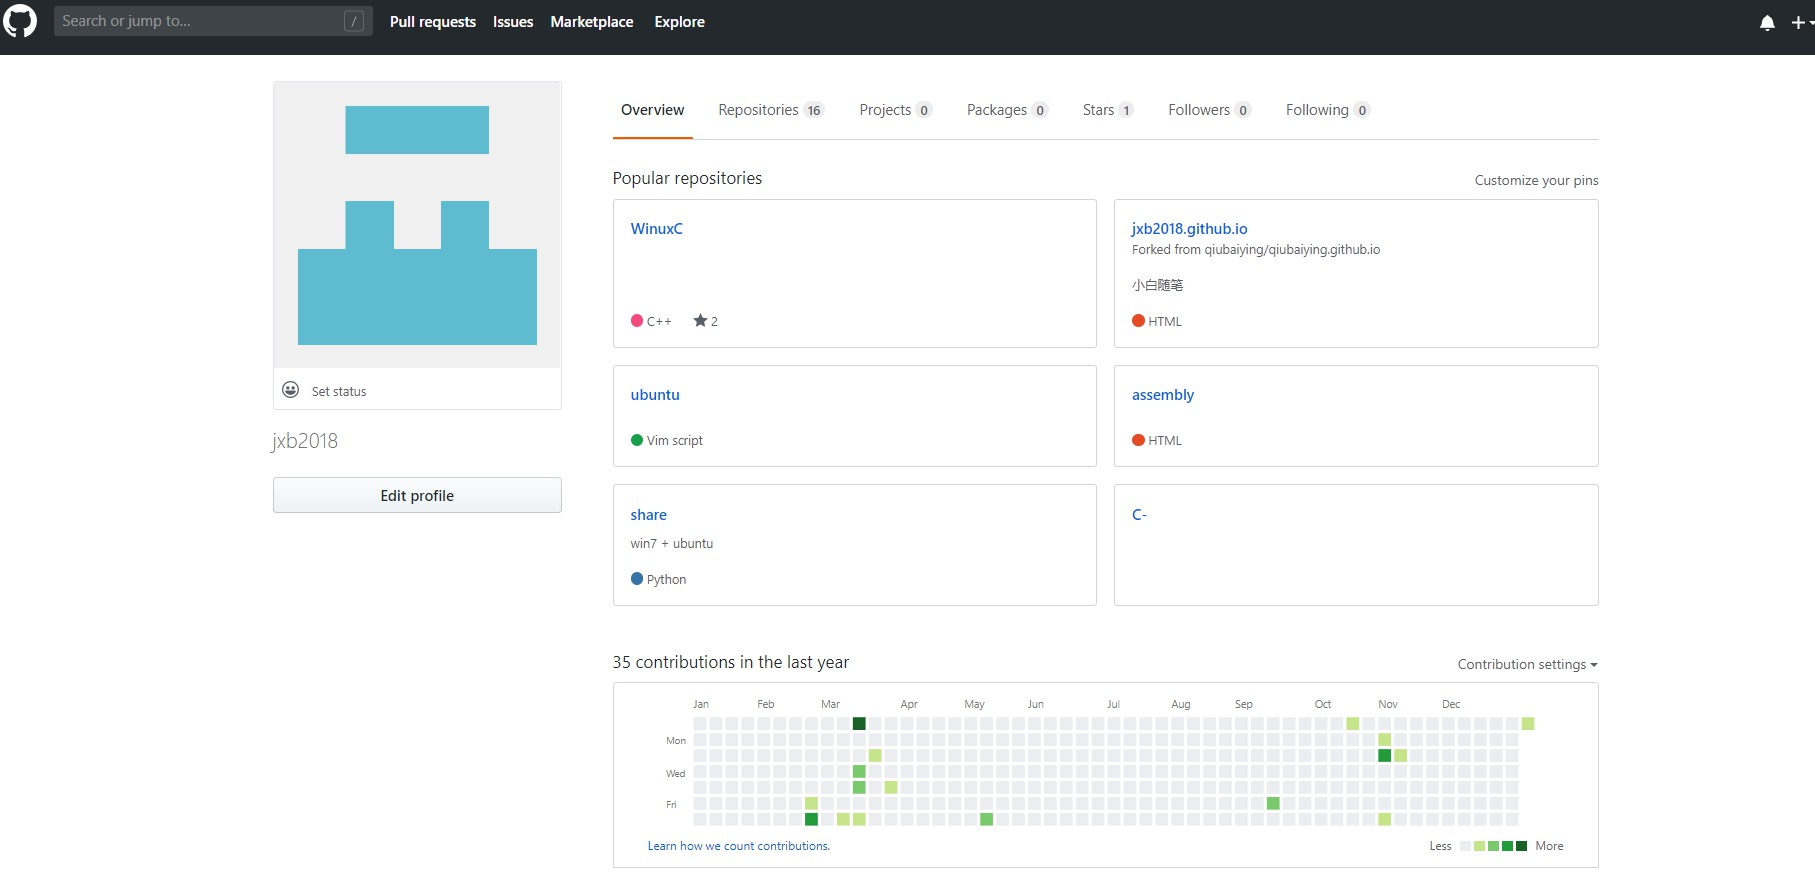
\includegraphics[scale=0.35]{github.jpg}
        \caption{Github个人主页}
        \label{fig:label}
        \end{figure}
    个人博客 
    \url{https://jxb2018.github.io/}\par
    \begin{figure}[ht]
        \centering
        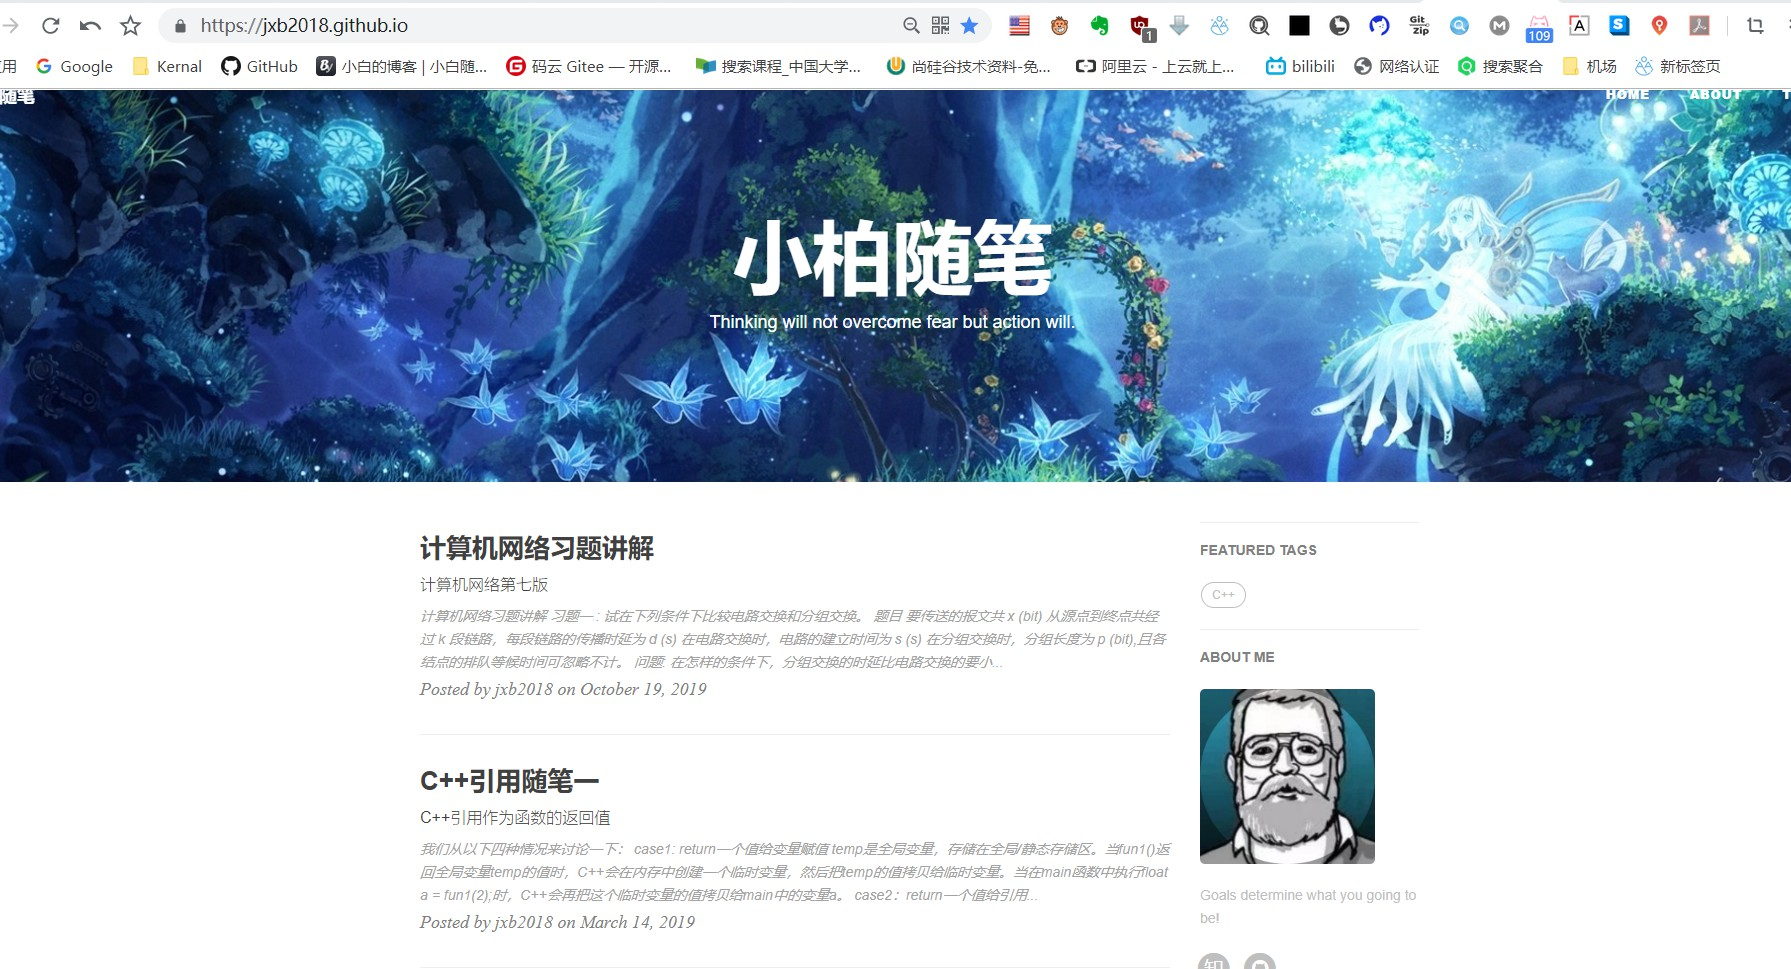
\includegraphics[scale=0.35]{gerenboke.jpg}
        \caption{Github个人博客}
        \label{fig:label}
        \end{figure}
    \newpage
    \item 观察者、哔哩哔哩
    \begin{figure}[ht]
        \centering
        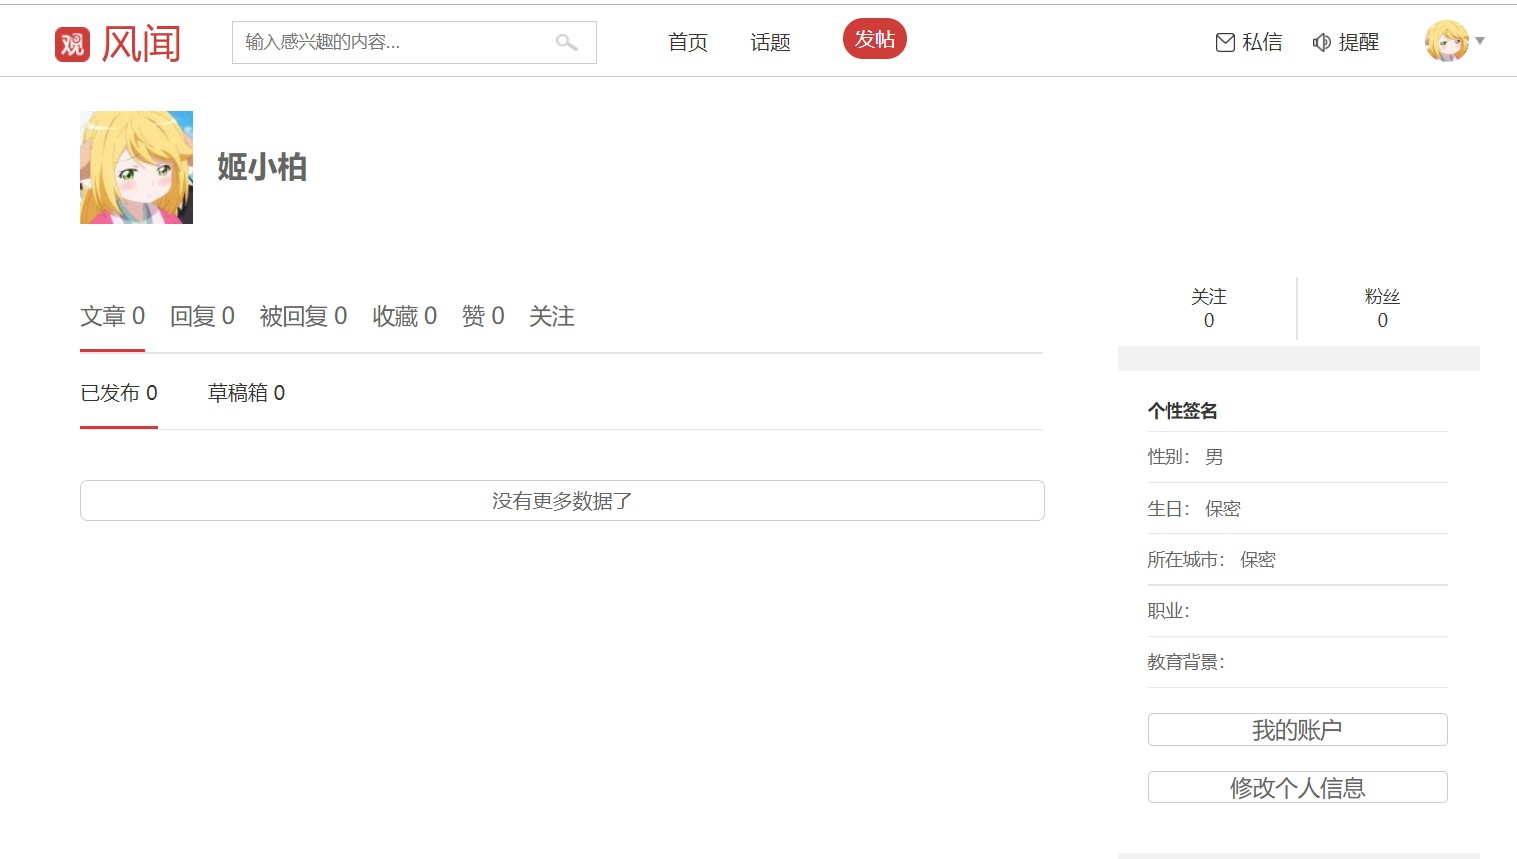
\includegraphics[scale=0.4]{guanchazhe.jpg}
        \caption{观察者网}
        \label{fig:label}
        \end{figure}
    \begin{figure}[ht]
        \centering
        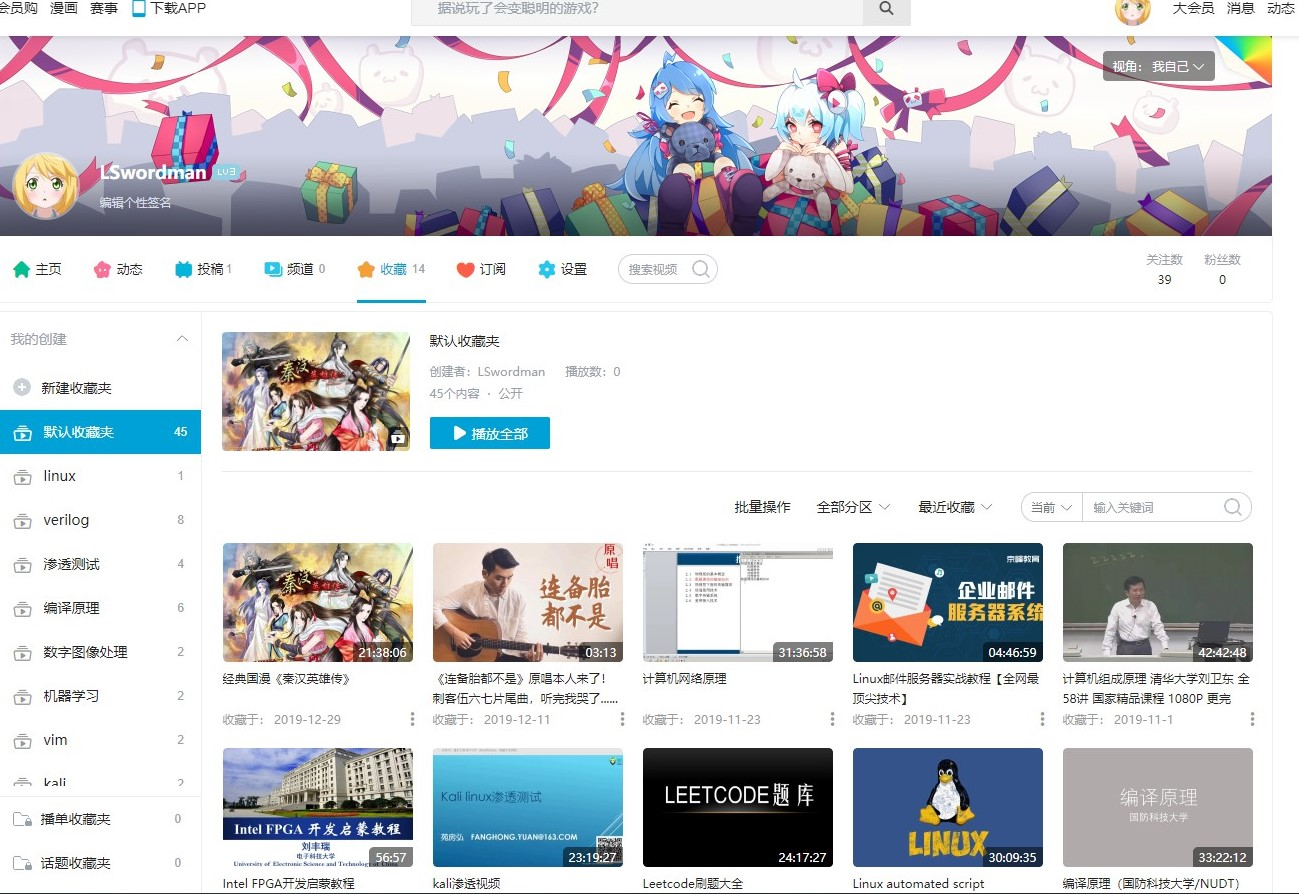
\includegraphics[scale=0.42]{bilibili.jpg}
        \caption{Bilibili}
        \label{fig:label}
        \end{figure}
    \newpage
    \item CSDN、博客园\par
    CSDN个人主页
    \url{https://me.csdn.net/weixin_43267246}\par
    \begin{figure}[ht]
        \centering
        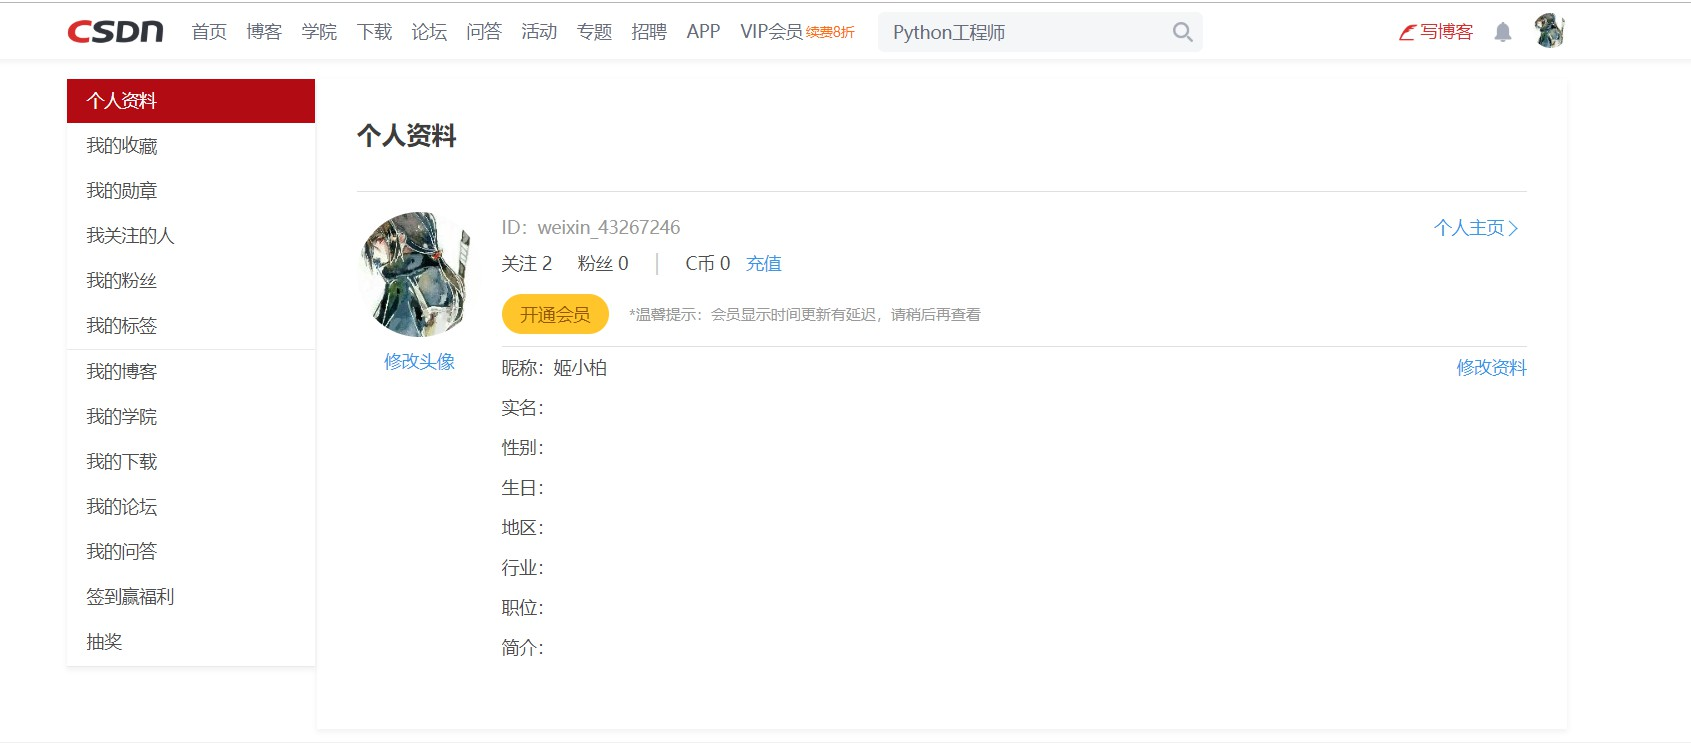
\includegraphics[scale=0.35]{csdn.jpg}
        \caption{CSDN}
        \label{fig:label}
        \end{figure}
    博客园个人主页
    \url{https://home.cnblogs.com/u/1916252/}\par
    \begin{figure}[ht]
        \centering
        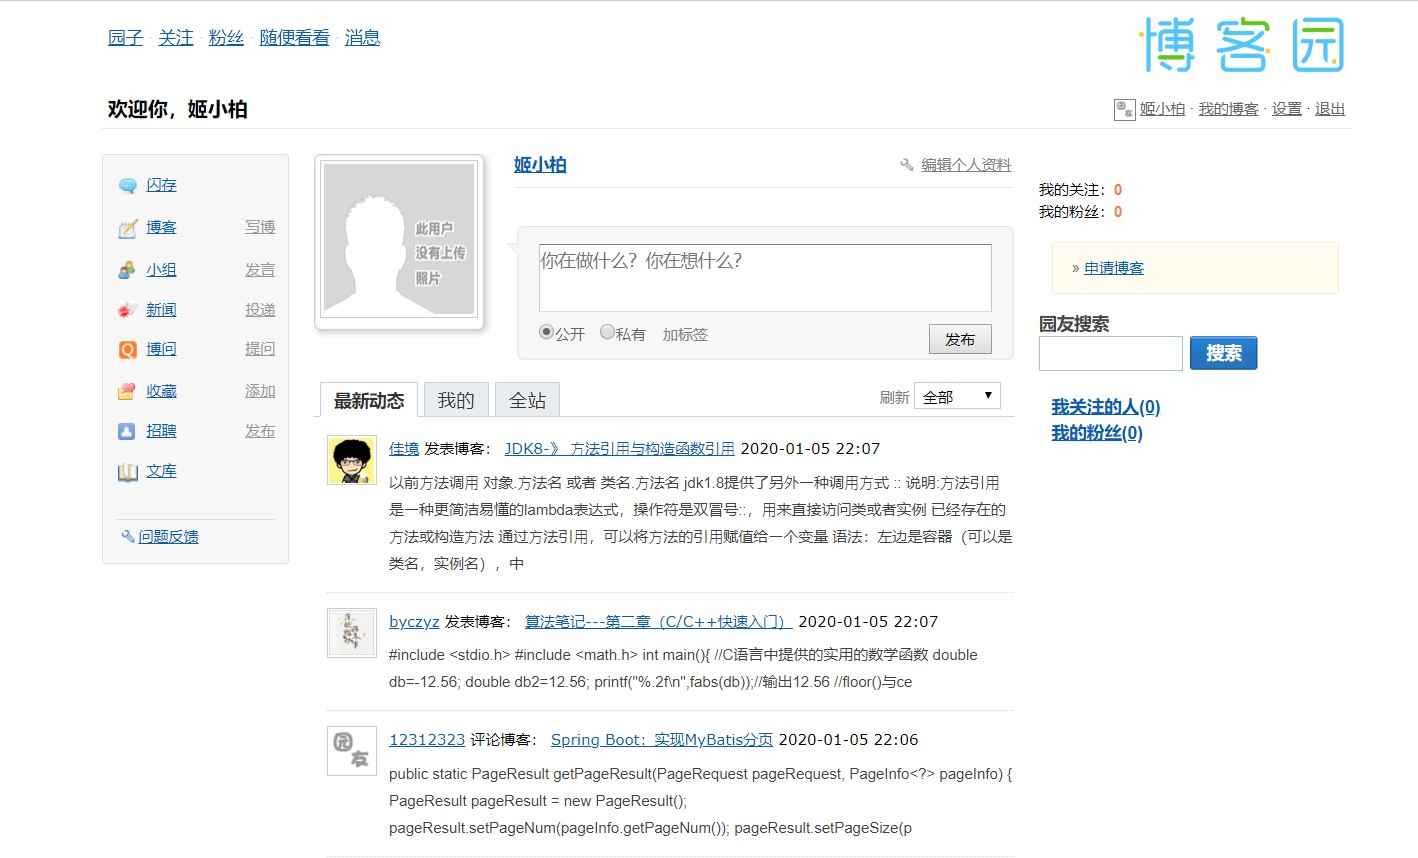
\includegraphics[scale=0.35]{bokeyuan.jpg}
        \caption{博客园}
        \label{fig:label}
        \end{figure}
    \newpage
    \item 小木虫、学习强国\par
    个人网址
    \url{http://muchong.com/bbs/space.php?uid=20410910}\par
    \begin{figure}[ht]
        \centering
        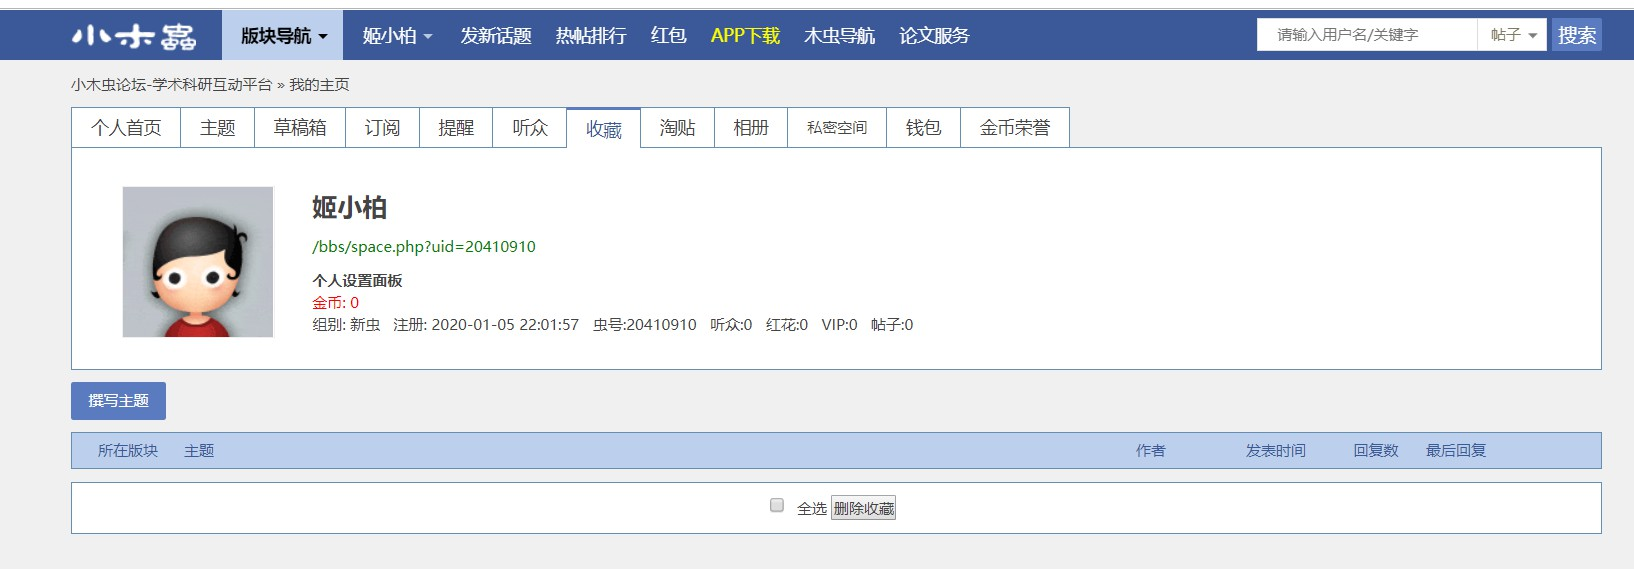
\includegraphics[scale=0.35]{xiaomuchong.jpg}
        \caption{小木虫}
        \label{fig:label}
        \end{figure}
    \begin{figure}[ht]
        \centering
        
\includegraphics[scale=0.35]{xuexi.jpg}
        \caption{学习强国}
        \label{fig:label}
        \end{figure}
\end{itemize}

\newpage










\hspace*{\fill} \\

\bibliographystyle{unsrt}
\bibliography{references}


\end{document}
